%!TEX root = vaisagh_thesis.tex

\chapter{Comparison of Information Based Perception against Controlled Experiments} % (fold)
\label{cha:speed_experiment_comparison}

Chapter~\ref{chapter:IBP} introduce an infromation based perception system and demonstrated it's effectiveness in helping existing motion planning systems produce more realistic behavior. In the chapter, results from simulations were compared against the controlled experiments conducted by Hu et al.~\cite{hunanThesis,HuNan2013}. In this section we present the results of two additional metrics --- the speed as a function of time and the trajectory length --- and compare the results produced against traditional RVO2, social force and the results produced in the experiment.

Regarding trajectory length, Hu's most significant finding was that, typically, the oncoming agent would travel a longer distance in order to avoid the oncoming group as shown in Table~\ref{tab:RealWorldTrajectoryLengths}. All three models produced similar dynamics as shown in Table~\ref{tab:SimulationTrajectoryLengths}.


\begin{table}[!t]

\centering
%     \begin{adjustbox}{width=\textwidth,center}
    % \begin{adjustbox}{center}
        \begin{tabular}{p{0.75in}   p{0.75in} p{0.75in} p{0.75in}}
            \hline
            \multicolumn{4}{c}{Trajectory Length Calculation from Experiments}  \\
            \hline
            \multicolumn{1}{c}{} &\multicolumn{1}{c}{Category 1 (\textbf{55\%})} &\multicolumn{1}{c}{Category 2 (40\%)}  &\multicolumn{1}{c}{Category 3 (5\%)} \\
            \hline
            \hline
            \multicolumn{1}{l}{Agent 1} & \multicolumn{1}{l}{10.0542} & \multicolumn{1}{l}{10.12006} & \multicolumn{1}{l}{10.15071}
            \\%\cline{2-5}
            \multicolumn{1}{l}{Agent 2} & \multicolumn{1}{l}{\textbf{10.238}}& \multicolumn{1}{l}{\textbf{10.27922}}& \multicolumn{1}{l}{10.15928}
            \\%\cline{2-5}
            \multicolumn{1}{l}{Agent 3} & \multicolumn{1}{l}{10.1126} & \multicolumn{1}{l}{10.0789} & \multicolumn{1}{l}{\textbf{10.18924}}
            \\%\cline{2-5}

            \hline
            \hline

        \end{tabular}
%     \end{adjustbox}
%     \vspace{ - 05 mm}
    \caption[Real world trajectory lengths~\cite{hunanThesis}]{Trajectory length according to experiments conducted by Nan~\cite{hunanThesis}. Category 1 refers to the movement of Agent 2 to the left of the group, category 2 to the movement of Agent 2 to the right of the group and category 3 to the movement of agent 2 through the middle of the oncoming group.}
    \label{tab:RealWorldTrajectoryLengths}
\end{table}

\begin{table}[!t]
\centering
%     \begin{adjustbox}{width=\textwidth,center}
    % \begin{adjustbox}{center}
        \begin{tabular}{p{0.75in}   p{0.75in} p{0.75in} p{0.75in} p{0.75in}}
            \hline
            \multicolumn{1}{c}{} & \multicolumn{1}{c}{Experiment (95\%)} & \multicolumn{1}{c}{RVO2+IBP} & \multicolumn{1}{c}{RVO2} & \multicolumn{1}{c}{Social Force}    \\
            \hline
            \hline
            \multicolumn{1}{l}{Agent 1}  & \multicolumn{1}{l}{10.087} & \multicolumn{1}{l}{9.925} & \multicolumn{1}{l}{9.925} & \multicolumn{1}{l}{10.003}
            \\%\cline{2-5}
            \multicolumn{1}{l}{Agent 2} & \multicolumn{1}{l}{10.259} & \multicolumn{1}{l}{12.132} & \multicolumn{1}{l}{11.833} & \multicolumn{1}{l}{11.831}
            \\%\cline{2-5}
            \multicolumn{1}{l}{Agent 3} & \multicolumn{1}{l}{10.096} & \multicolumn{1}{l}{9.925} & \multicolumn{1}{l}{9.925} & \multicolumn{1}{l}{10.003}
            \\%\cline{2-5}

            \hline
            \hline
        \end{tabular}
%     \end{adjustbox}
%     \vspace{ - 05 mm}
    \caption[Simulation trajectory lengths]{This table shows the trajectory length obtained for the simulation of the experimental scenario in~\cite{hunanThesis}. The first column lists the average of category 1 and 2 which together comprised 95\% of the real world experiment data of~\cite{hunanThesis}.}
    \label{tab:SimulationTrajectoryLengths}
\end{table}

Figure~\ref{fig:SpeedIBPPlot} shows the development of speed against time for the three models that were considered. Hu et al observed that one of the problems with existing motion planning systems was that there was a significant slowing of agent 2 when it gets closer to the other agents; whereas in the real world results all three participants maintained their speed. When RVO2 is used with IBP there is a dip in speed of participant 2 but this lasts for less than a second as shown in Fig~\ref{fig:SpeedIBPPlot}. For the rest of the simulation, the agent maintains its speed. As seen in the figure, this isn't the case with RVO2 with a traditional sensor range.



\begin{figure}[!b]
  \centering
  \subfloat[Agent 2]{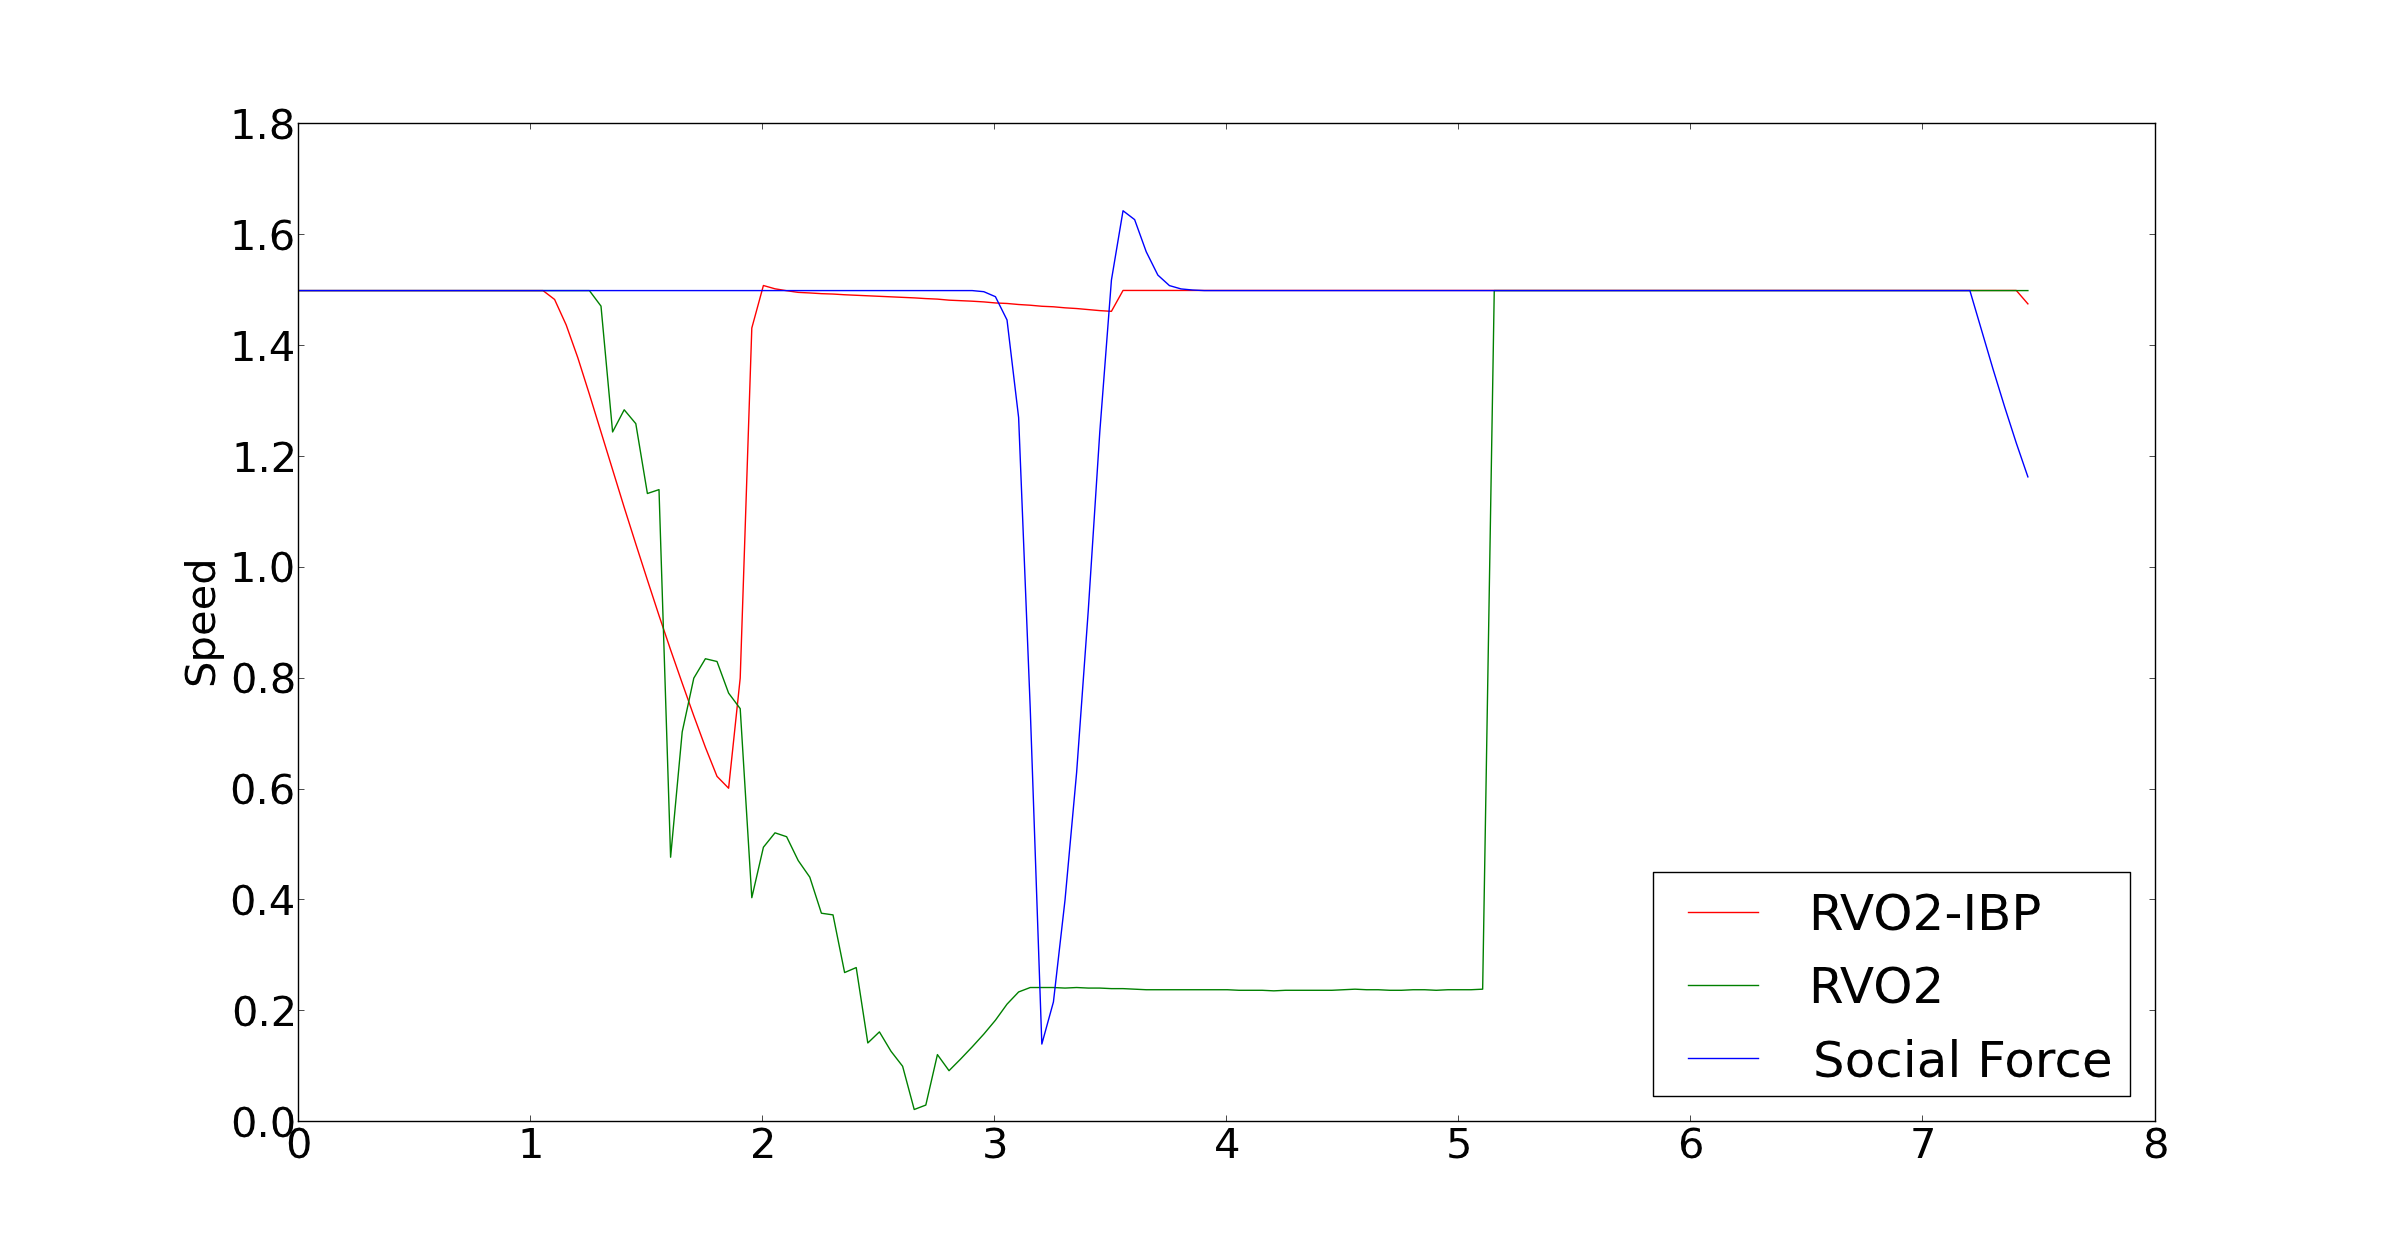
\includegraphics[width=0.60\textwidth]{InfoBasedPerception/SpeedPlot-agent2.png}}
   \\
   \subfloat[Agent 1]{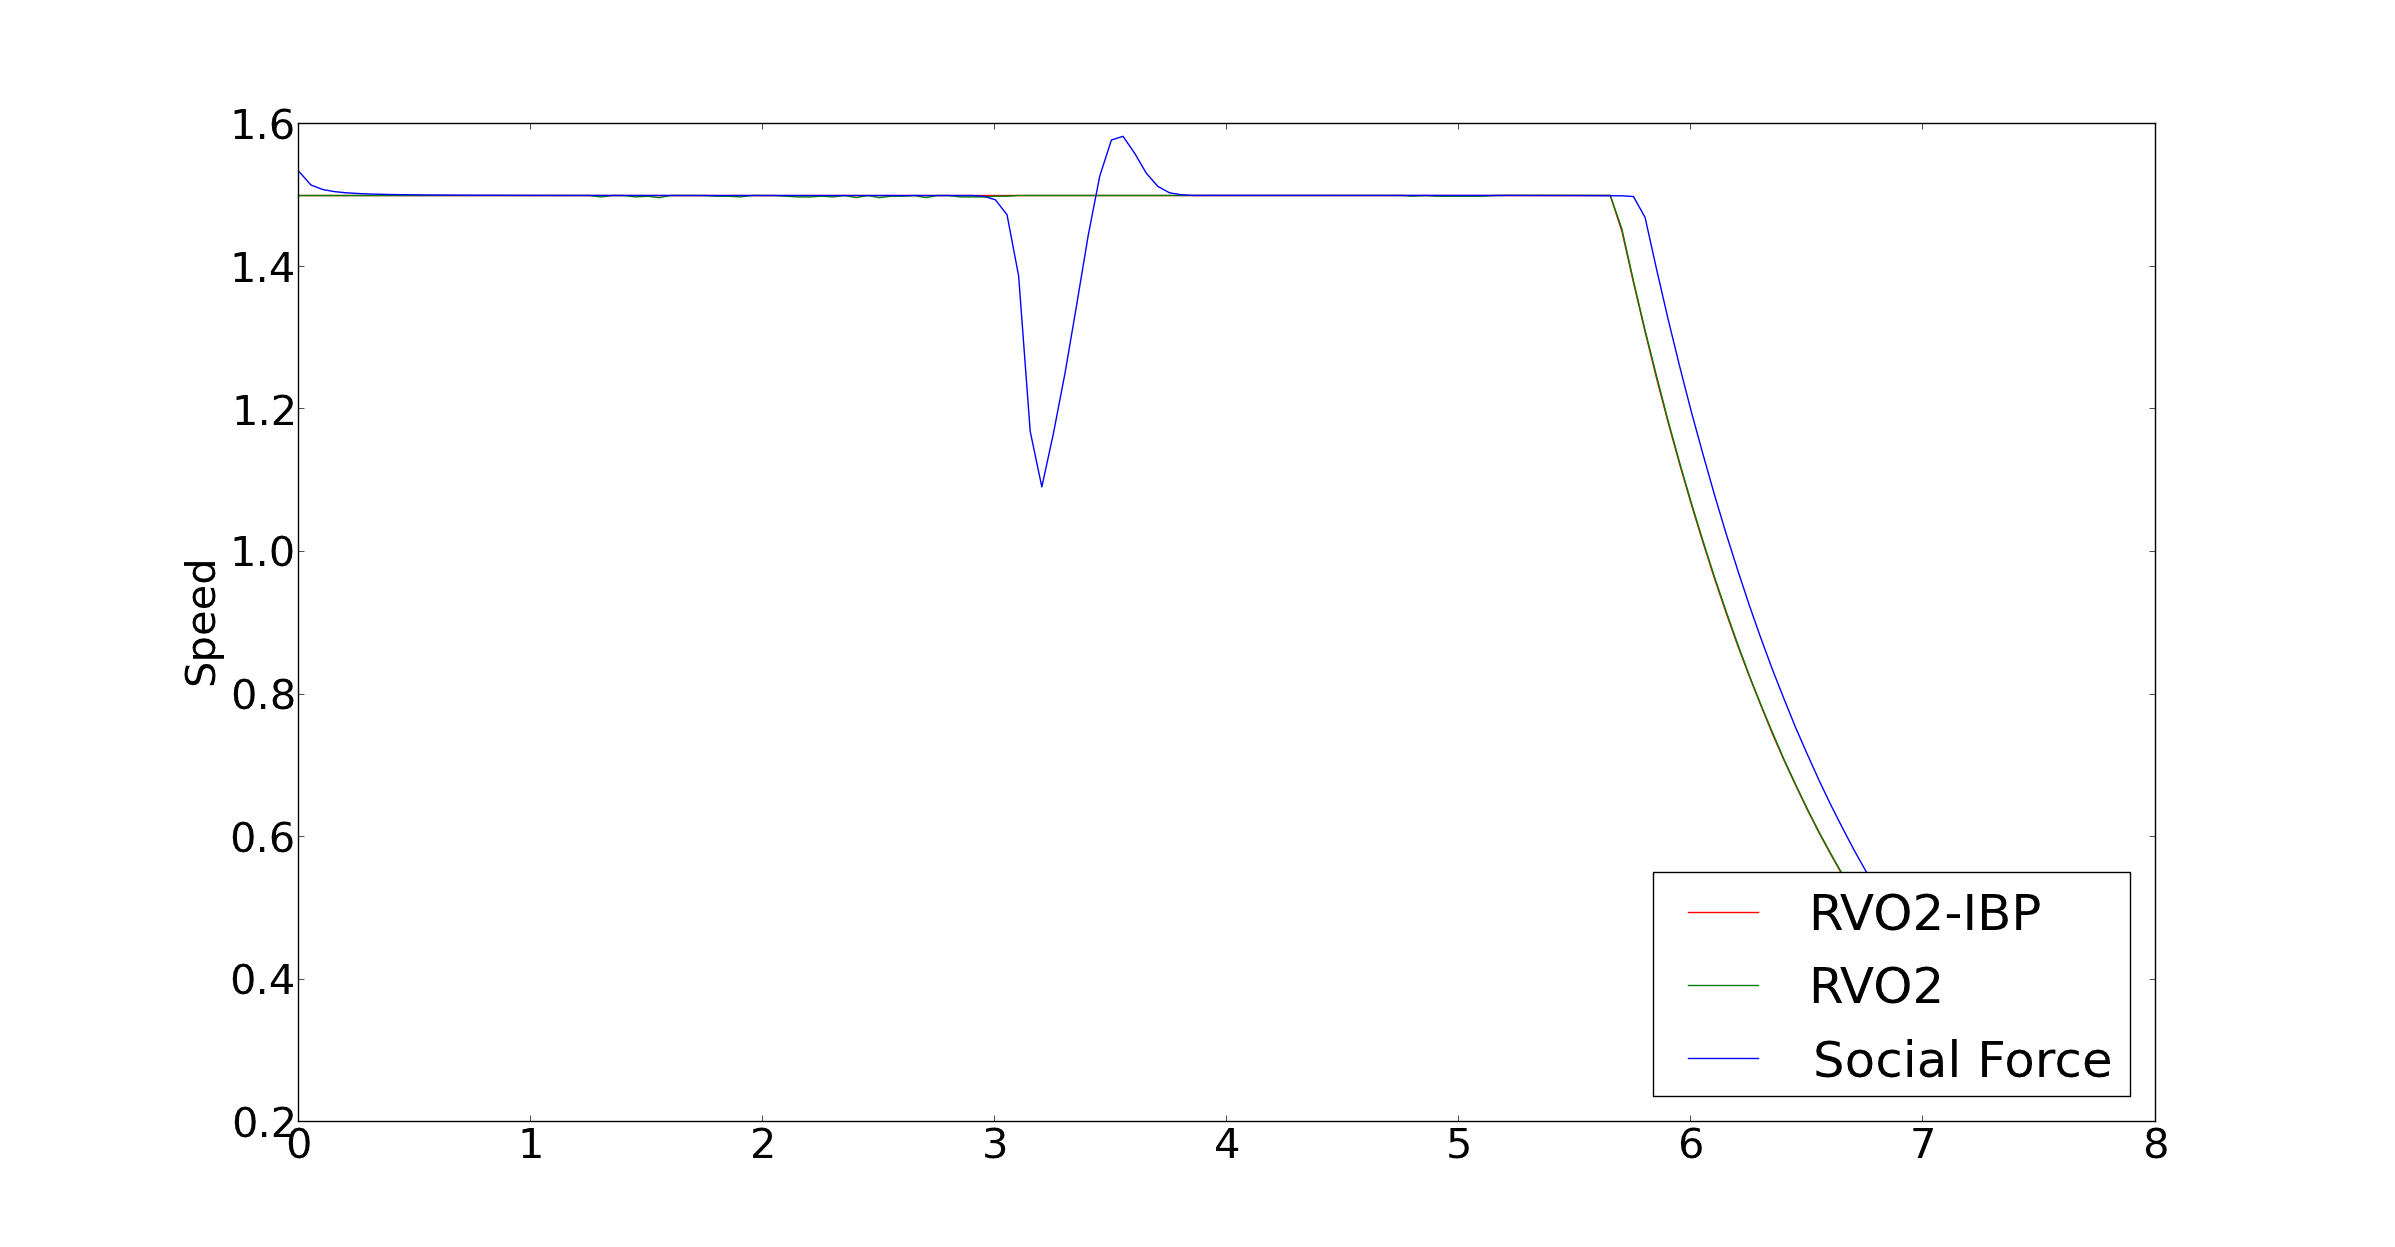
\includegraphics[width=0.48\textwidth]{InfoBasedPerception/SpeedPlot-agent1.png}}
   \hspace{1pt}
    \subfloat[Agent 3]{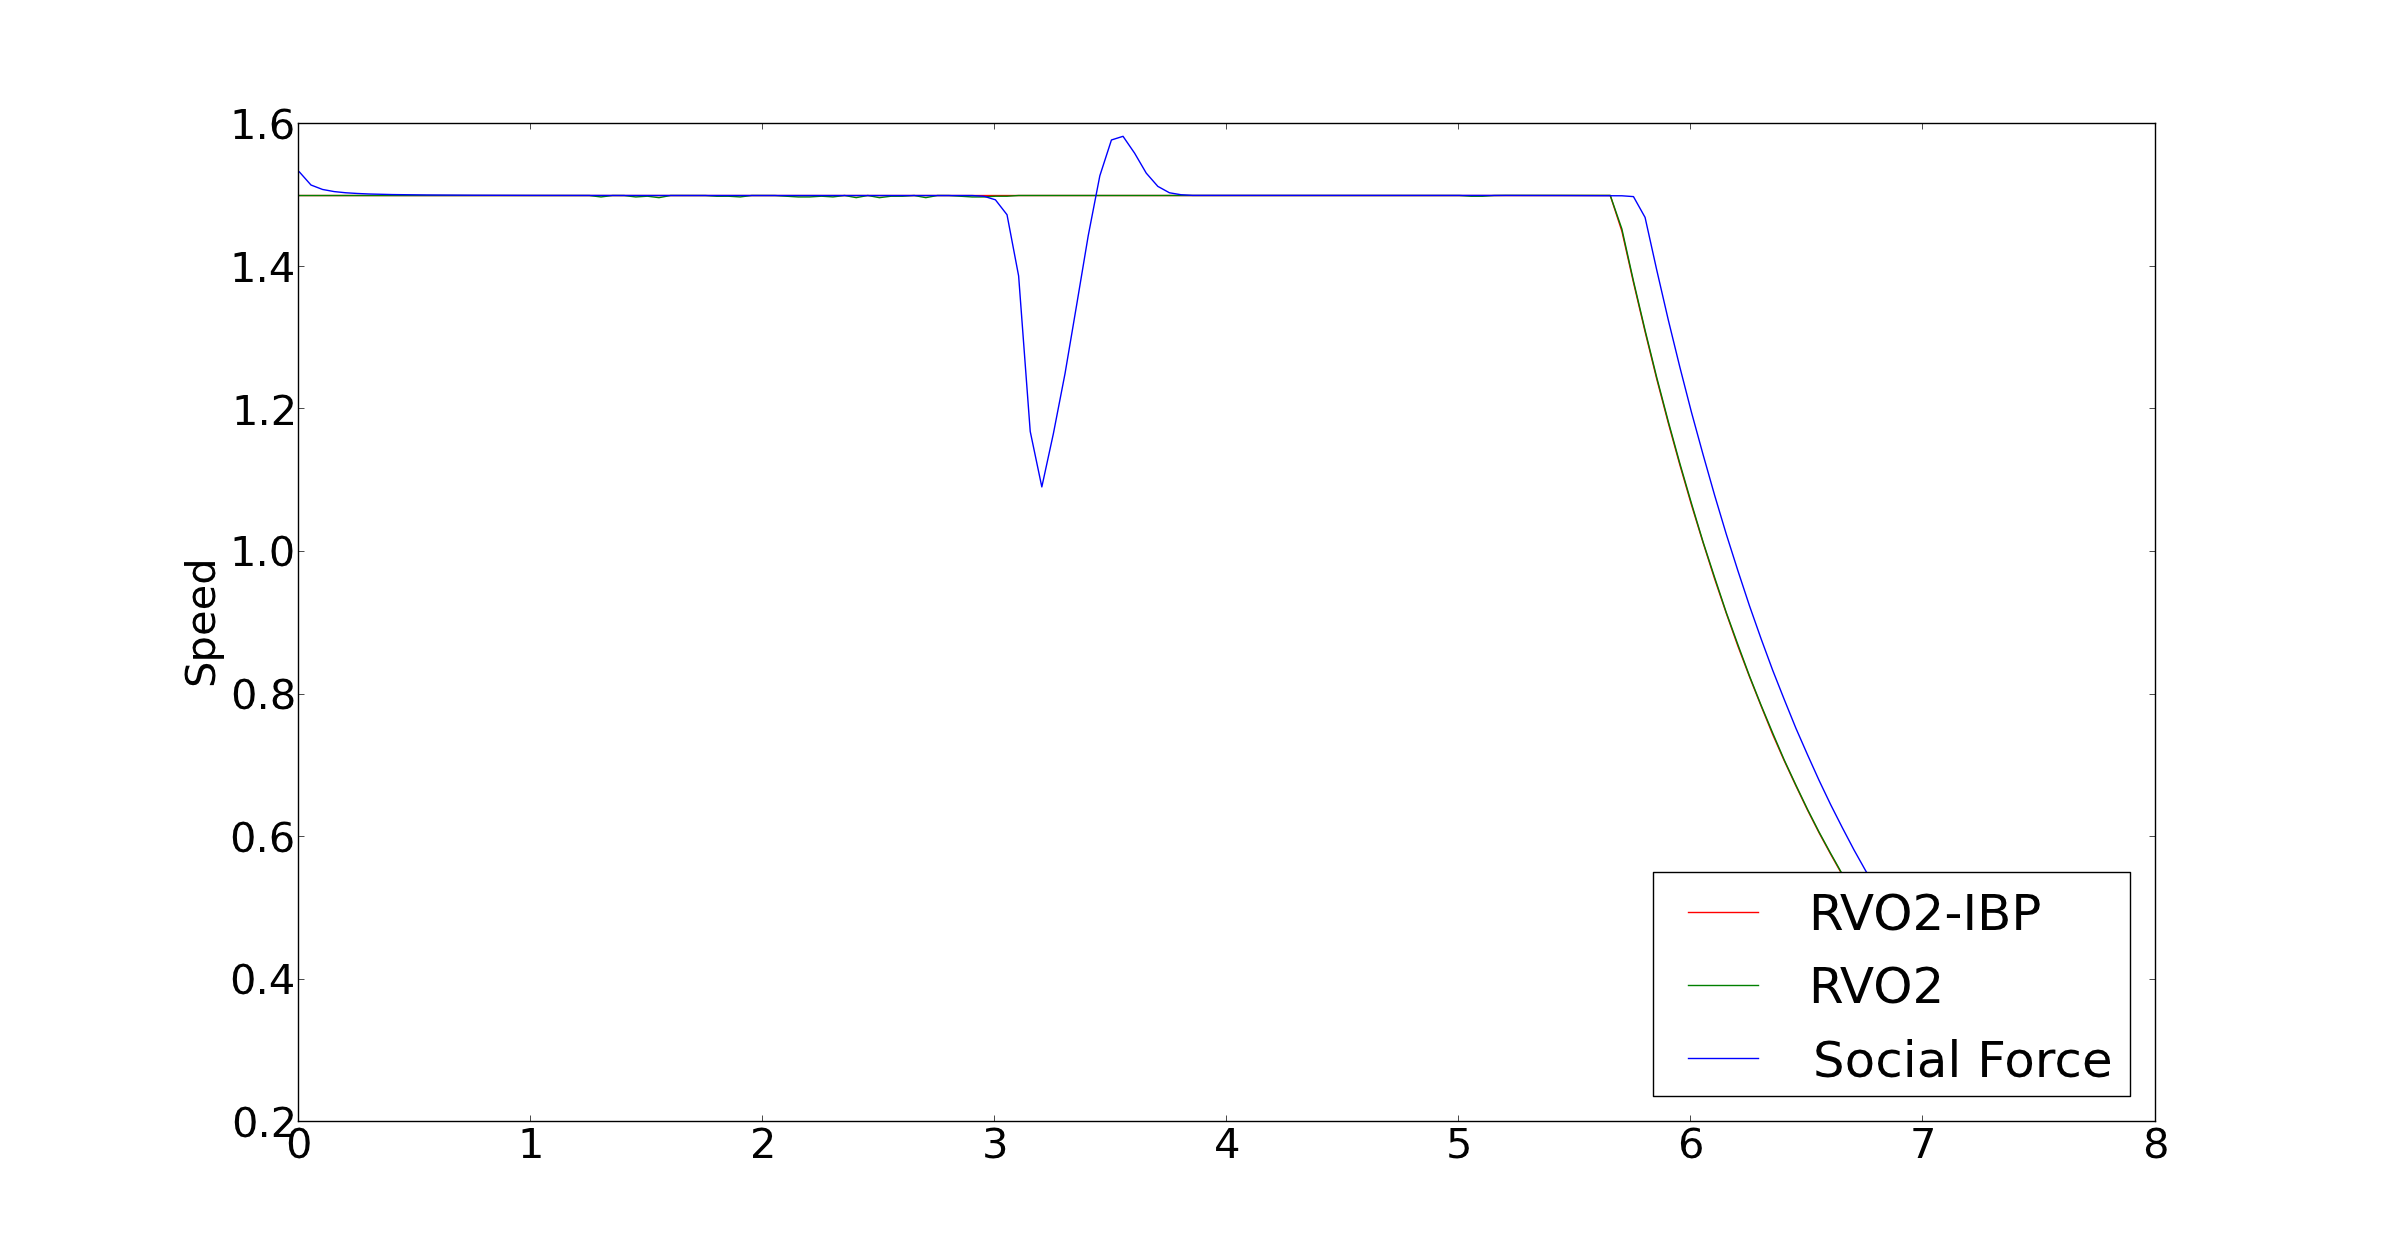
\includegraphics[width=0.48\textwidth]{InfoBasedPerception/SpeedPlot-agent3.png}}
  \caption[Speed plot comparison]{Hu et al. observed that real world participants reached a stable average speed of $1.5 ms^{-1}$ and maintained that speed for the duration of the experiment run. This figure shows the results produced by RVO2, Social Force and IBP-RVO2. While Social Force seems to produce results that agrees with the experiment, Agent 2 seems to slow down considerably when traditional RVO2 is used. However, when used with IBP, there is only an instantaneous drop in velocity (for less than a second) as in Social Force.}
  \label{fig:SpeedIBPPlot}
\end{figure}

% chapter speed_experiment_comparison (end)